\documentclass{article} % For LaTeX2e
\usepackage{final_project,times}
\usepackage{graphicx}
\usepackage{subcaption}
%\documentstyle[nips12submit_09,times,art10]{article} % For LaTeX 2.09


\title{Bayesian Non-Parametrics and Dirichlet Process Clustering Techniques}


\author{
Radhika Anand, Dipesh Gautam, Princeton Lee\thanks{ Use footnote for providing further information
about author (webpage, alternative address)} \\
Department of Statistical Sciences\\
Duke University\\
}

\newcommand{\fix}{\marginpar{FIX}}
\newcommand{\new}{\marginpar{NEW}}

\nipsfinalcopy

\begin{document}


\maketitle

\begin{abstract}

\end{abstract}

\section{Introduction}
Standard clustering algorithms like K-Means and Gaussian Mixture Models require us to know the total number of clusters a-priori. This has two problems:
\begin{itemize}
\item We do not always know the number of clusters a-priori
\item Most real-world problems don’t have a fixed number of clusters
\end{itemize}
This brings us to a class of algorithms called Non-Parametric Bayes, which assumes that true dimensionality is unbounded and allows the parameters to grow with growing data. It doesn’t require a prior specification of the number of latent clusters, which it instead infers from the data itself.

Commonly studied non-parametric clustering techniques include:
\begin{enumerate}
\item Chinese Restaurant Process
\item Polya Urn Model
\item Dirichlet Process
\item Indian Buffet Process (for feature allocation)
\end{enumerate}


\section{Discussion of different clustering models}
\subsection{Chinese Restaurant Process}
Consider data points as customers who visit a restaurant and clusters as tables in that restaurant. CRP is based on the idea that there are infinite number of tables in the restaurant and infinite number of seats at each table. The first customer sits at a table. The (n+1)st customer then sits at a new table with probability $\frac{\alpha}{(n+\alpha)}$ and on an occupied table with probability $\frac{n_k}{(n+\alpha)}$, where $n_k$ is the number of customers occupying table k.

Points to note:
\begin{enumerate}
\item The more the customers at a table, the more probable it is that the next customer will join that table. This is the rich-get-richer property.
\item Probability of a new table (cluster) is proportional to $\alpha$. Thus, we consider $\alpha$ as a dispersion parameter which determines the total number of clusters. The higher the $\alpha$, the higher is the number of clusters in a given set of data.
\end{enumerate}
Finally, CRP specifies a distribution over partitions/table assignments but does not assign parameters to tables (which can be done by the Polya Urn Model as in the next section).

Fig. \ref{fig:crp} below shows how the total number of detected clusters increases with increasing $\alpha$ value.
\begin{figure}[h]
\begin{center}
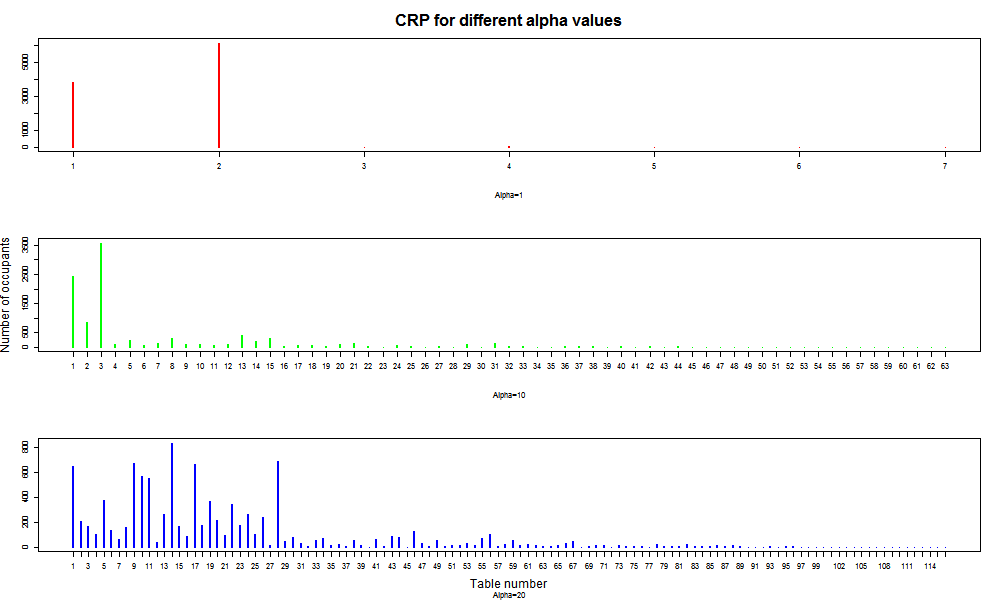
\includegraphics[width=\linewidth]{crp.png}
\caption{Number of distinct tables for different $\alpha$ values}
%\fbox{\rule[-.5cm]{0cm}{4cm} \rule[-.5cm]{4cm}{0cm}}
\label{fig:crp}
\end{center}
\end{figure}


\subsection{Polya Urn Model}
Consider data points as balls in an urn and their colors as the clusters they belong to. We now pick a ball from the urn, note its color and drop that ball and another ball of the same color back into the urn.

Thus, it is similar to CRP in that it follows the rich-get-richer property and has $\alpha$ as the dispersion parameter.

Further, it not only specifies a distribution over partitions but also assigns parameters to them. It is like a distribution over distributions as can be visualized from the various runs of the same Polya Urn Model in the plots below. This brings us to the Dirichlet Process.

Fig. \ref{fig:polya} shows the density of colors in the urn for several runs. We use standard normal as the base color distribution. Thus, as $\alpha$ increases i.e. we sample more and more new colors from the base distribution, we see that the plots tend towards standard normal i.e. they approach the base distribution.
\begin{figure}
  \centering
  \caption{Density of colors for different $\alpha$ values with standard normal as base distribution}
\label{fig:polya}
  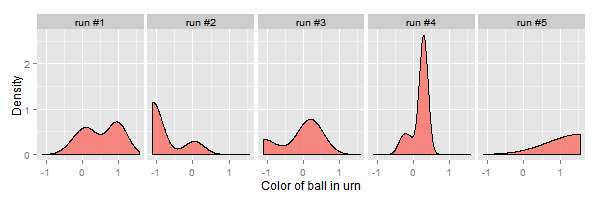
\includegraphics[width=\linewidth]{polya-urn-1.png}
  \subcaption{}
  \label{fig:polya1}
  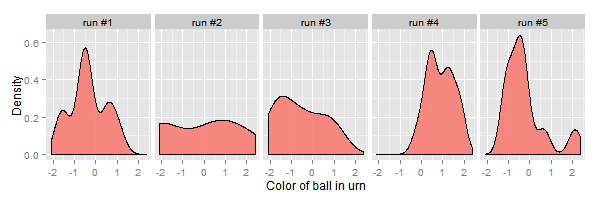
\includegraphics[width=\linewidth]{polya-urn-5.png}
  \subcaption{}
  \label{fig:polya5}
  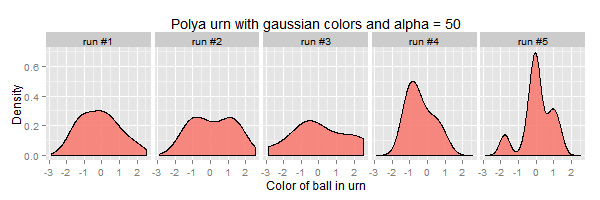
\includegraphics[width=\linewidth]{polya-urn-50.png}
  \subcaption{}
  \label{fig:polya50}
\end{figure}

\subsection{Dirichlet Process Mixture Models}
Suppose we have multivariate, real-valued data y1,…,yn, which is exchangeable, a DPMM is defined as follows:
\begin{eqnarray*}
y_i|\theta_i \sim F(\theta_i)\\
\theta_i|G \sim G\\
G \sim D(G_0, \alpha)
\end{eqnarray*}
i.e., we model the distribution from which $y_i$'s are drawn as a mixture of distributions of the form $F(\theta)$, which is normal for a Gaussian DPMM, with $G$ as the mixing distribution over parameters $\theta$. Further, the prior over $G$ is a Dirichlet Process with base distribution $G_0$ and dispersion parameter $\alpha$.


\section{Method}
\section{Results}
\section{Discussion}
\section{Conclusions}

\subsection{Style}

Papers describing final project should be up to four pages long (not including bibliography). They should contain an abstract, introduction, related work, methods, results, discussion, and conclusion section, and figures and tables where necessary, and a bibliography. These papers are due on April 16th in class.


\subsection{Retrieval of style files}

The formatting instructions contained in these style files are summarized in
sections \ref{gen_inst}, \ref{headings}, and \ref{others} below.

\section{General formatting instructions}
\label{gen_inst}

The text must be confined within a rectangle 5.5~inches (33~picas) wide and
9~inches (54~picas) long. The left margin is 1.5~inch (9~picas).
Use 10~point type with a vertical spacing of 11~points. Times New Roman is the
preferred typeface throughout. Paragraphs are separated by 1/2~line space,
with no indentation.

Paper title is 17~point, initial caps/lower case, bold, centered between
2~horizontal rules. Top rule is 4~points thick and bottom rule is 1~point
thick. Allow 1/4~inch space above and below title to rules. All pages should
start at 1~inch (6~picas) from the top of the page.


\section{Headings: first level}
\label{headings}

First level headings are lower case (except for first word and proper nouns),
flush left, bold and in point size 12. One line space before the first level
heading and 1/2~line space after the first level heading.

\subsection{Headings: second level}

Second level headings are lower case (except for first word and proper nouns),
flush left, bold and in point size 10. One line space before the second level
heading and 1/2~line space after the second level heading.

\subsubsection{Headings: third level}

Third level headings are lower case (except for first word and proper nouns),
flush left, bold and in point size 10. One line space before the third level
heading and 1/2~line space after the third level heading.

\section{Citations, figures, tables, references}
\label{others}

These instructions apply to everyone, regardless of the formatter being used.

\subsection{Citations within the text}

Citations within the text should be numbered consecutively. The corresponding
number is to appear enclosed in square brackets, such as [1] or [2]-[5]. The
corresponding references are to be listed in the same order at the end of the
paper, in the \textbf{References} section. (Note: the standard
\textsc{Bib\TeX} style \texttt{unsrt} produces this.) As to the format of the
references themselves, any style is acceptable as long as it is used
consistently.

\subsection{Figures}

All artwork must be neat, clean, and legible. Lines should be dark
enough for purposes of reproduction; art work should not be
hand-drawn. The figure number and caption always appear after the
figure. Place one line space before the figure caption, and one line
space after the figure. The figure caption is lower case (except for
first word and proper nouns); figures are numbered consecutively.

Make sure the figure caption does not get separated from the figure.
Leave sufficient space to avoid splitting the figure and figure caption.

\begin{figure}[h]
\begin{center}
%\framebox[4.0in]{$\;$}
\fbox{\rule[-.5cm]{0cm}{4cm} \rule[-.5cm]{4cm}{0cm}}
\end{center}
\caption{Sample figure caption.}
\end{figure}

\subsection{Tables}

All tables must be centered, neat, clean and legible. Do not use hand-drawn
tables. The table number and title always appear before the table. See
Table~\ref{sample-table}.

Place one line space before the table title, one line space after the table
title, and one line space after the table. The table title must be lower case
(except for first word and proper nouns); tables are numbered consecutively.

\begin{table}[t]
\caption{Sample table title}
\label{sample-table}
\begin{center}
\begin{tabular}{ll}
\multicolumn{1}{c}{\bf PART}  &\multicolumn{1}{c}{\bf DESCRIPTION}
\\ \hline \\
Dendrite         &Input terminal \\
Axon             &Output terminal \\
Soma             &Cell body (contains cell nucleus) \\
\end{tabular}
\end{center}
\end{table}

\section{Final instructions}
Do not change any aspects of the formatting parameters in the style
files.  In particular, do not modify the width or length of the
rectangle the text should fit into, and do not change font sizes.
Please note that pages should be numbered.

\section{Preparing PostScript or PDF files}

Please prepare PostScript or PDF files with paper size ``US Letter'', and
not, for example, ``A4''. The -t
letter option on dvips will produce US Letter files.

\begin{itemize}

\item Consider directly generating PDF files using \verb+pdflatex+

\item Otherwise, please generate your PostScript and PDF files with the following commands:
\begin{verbatim}
dvips mypaper.dvi -t letter -Ppdf -G0 -o mypaper.ps
ps2pdf mypaper.ps mypaper.pdf
\end{verbatim}
\end{itemize}


\subsubsection*{Acknowledgments}

Use unnumbered third level headings for the acknowledgments. All
acknowledgments go at the end of the paper.

\subsubsection*{References}

References follow the acknowledgments. Use unnumbered third level heading for
the references. Any choice of citation style is acceptable as long as you are
consistent. CITE A LOT. Any unreferenced methods, prior work, or biological phenomenon, unless it is textbook-common, will be penalized.

\small{
[1] Alexander, J.A. \& Mozer, M.C. (1995) Template-based algorithms
for connectionist rule extraction. In G. Tesauro, D. S. Touretzky
and T.K. Leen (eds.), {\it Advances in Neural Information Processing
Systems 7}, pp. 609-616. Cambridge, MA: MIT Press.

[2] Bower, J.M. \& Beeman, D. (1995) {\it The Book of GENESIS: Exploring
Realistic Neural Models with the GEneral NEural SImulation System.}
New York: TELOS/Springer-Verlag.

[3] Hasselmo, M.E., Schnell, E. \& Barkai, E. (1995) Dynamics of learning
and recall at excitatory recurrent synapses and cholinergic modulation
in rat hippocampal region CA3. {\it Journal of Neuroscience}
{\bf 15}(7):5249-5262.
}

\end{document}
